This chapter contains the implementation of the protocol designed in Chapter \ref{cha:protocolDesign}. 

First, the classes used in the implementation are shown and explained. Then important parts of the code are explained.
 

\section{General}
The implementation is written in C++. The development of the solution is done in two man teams, using pair programming. Git is used for version control.

\section{Classes}
The solution contains two different running applications. The main node and the sensor nodes. There are two sets of code due to the different requirements of the nodes. For example, the main node does not have a sensor, so it should not be able to handle a sensor, and therefore does not contain the classes used for sensors.

This section contains the classes contained in each application.

\subsubsection*{Main node}
The main node is a Raspberry Pi device, running the Raspbian operating system. The classes in the main node application is seen on Figure \ref{fig:mainnodeClass}.
The main node pairs nodes, send requests, and handles receiving and handling data.

\begin{figure}[h!]
\centering
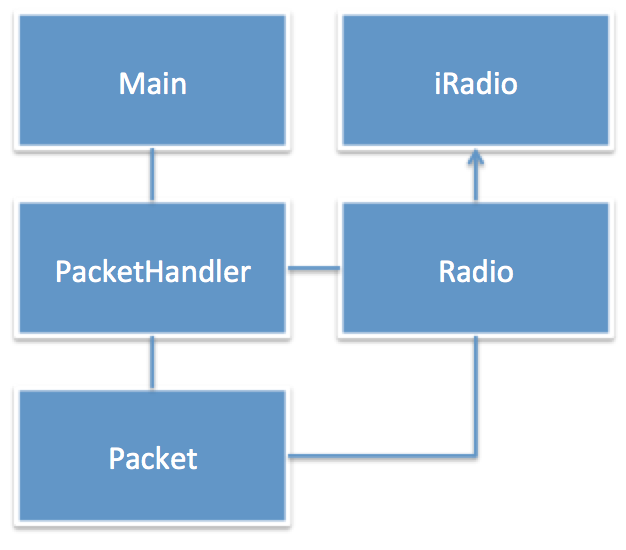
\includegraphics[width=0.65\textwidth]{chapters/implementation/figures/mainnodeClass.png}
\caption{Classes used in the main node.}
\label{fig:mainnodeClass}
\end{figure}



\subsubsection*{Sensor nodes}
The platform on the sensor nodes are comprised of Arduino Uno or Mega. The difference in the two platforms are the pins used with the sensors and radio modules. Besides that, the code on the platforms are the same. The sensor nodes handles receiving and sending requests, reading and sending sensor data, and relaying data through nodes until they arrive at the main node. 

The classes used in the nodes are seen on Figure \ref{fig:nodeClass}.
\begin{figure}[h!]
\centering
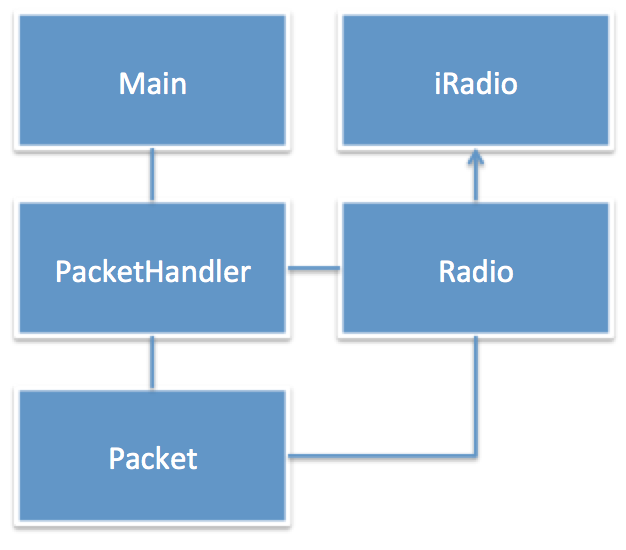
\includegraphics[width=0.85\textwidth]{chapters/implementation/figures/nodeClass.png}
\caption{Classes used in nodes.}
\label{fig:nodeClass}
\end{figure}


\subsubsection*{Class descriptions}
This section contains explanations about the classes used in the nodes.

\begin{description}
\item[Node] \hfill \\
The \textit{Node} class is the entrypoint in the application.
Contains one or more \textit{iSensor}s, and a \textit{iRadio} object that are instantiated when the code is run.

The \textit{Node} class determines what action to take when a packet is received. This happens in the method \textit{void determineAction(String packet)}. 
If data is received from another sensor node that should be relayed, the \textit{Node} begins sending data until an acknowledgement is received. The methods on the \textit{iRadio} object is used for listening and sending.
If data is needed for a packet, for example when a request is received, the \textit{Node} class fetches data from the sensor, and creates the packet that needs to be sent, and makes sure that the data is sent.

\item[iRadio and iSensor] \hfill \\
The \textit{iSensor} and \textit{iRadio} interfaces are used to create a certain way that all sensors and radio module classes should work. This means that replacing or adding a new sensor or using another radio module is not a problem, as the rest of the application knows that the radio is able to send and receive, and the sensor is able to return a value. 
It is not necessary to know how it is done, only that it is possible. These interfaces are used to set a standard on how to communicate with them, whether it is a moisture sensor or a pH sensor.

Every type of radio or sensor added to the node will inherit from these interfaces.


\textit{iSensor} only contains the method \textit{int read()}, that returns the value of the sensor.

\textit{iRadio} contains the methods:
\begin{description}
\item[void broadcast(String packet)] sends a packet
\item[String beginListening()] begins listening
\item[String listenFor(int ms)] begins listening, but stops listening after 'ms' ms
\end{description}

\item[Sensor] \hfill \\
The \textit{Sensor} class can be used for multiple sensors, as long as the sensor class inherits from \textit{iSensor}. This class' job is to read data from a sensor on the node, handle this data, and return it to the class that requested this data.

In the solution, as the moisture sensor is used, the sensor class is called \textit{MoistureSensor}. This class can only be found on the sensor nodes, and not on the main node.


\item[Radio] \hfill \\
The \textit{Radio} class handles the radio communication. Types of this class should inherit from the \textit{iRadio} interface. The \textit{Radio} class returns a packet in string format when one is received. It is also able to send packets given from other classes.

\item[Packet] \hfill \\
The class \textit{Packet} contains the ability to parse a packet from a string to a \textit{Packet} object, along with the properties required to further handle the packet. This includes the type, and possibly sensor values, from/to values or an identifier from the main node.

Instances of this class is created and used in the \textit{Node} class.

This class contains the public methods:
\begin{description}
\item[Packet(String packetString)] Create a packet from a string. Used when radio receives packet.
\item[Packet(String from, String to, int sensorValue)] Creates packet with sender, receiver and a value
\item[String stringRepresentation()] Returns a string representation of the packet. Used for broadcasting from the radio
\end{description}

\end{description}


\section{Code?}